\documentclass[../BTL.tex]{subfiles}
\begin{document}

\section{Mô hình hệ gợi ý}
Nội dung dành riêng.

\section{Hệ thống xử lý dữ liệu}
Hệ thống xử lý dữ liệu của đề tài gồm mười một dịch vụ (service), mỗi dịch vụ đảm nhận một vai trò xác định trong đường ống xử lý (pipeline) từ khi tiếp nhận sự kiện từ người dùng đến khi lưu trữ kết quả phân tích. Phần này trình bày kiến trúc tổng quan của hệ thống, luồng dữ liệu chi tiết giữa các thành phần, và cách triển khai từng module xử lý.

\subsection{Kiến trúc tổng quan}
Hệ thống gồm mười một container được tổ chức như sau:

\begin{table}[H]
\centering
\label{tab:services}
\begin{tabular}{|l|l|}
\hline
\textbf{Service} & \textbf{Vai trò} \\
\hline
\textbf{api} & Tiếp nhận sự kiện, trả về kết quả gợi ý \\
\hline
\textbf{spark-master} & Điều phối tác vụ (job) Spark trong cụm (cluster) \\
\hline
\textbf{spark-worker-1} & Nút công nhân (worker) chạy tác vụ (task) Spark \\
\hline
\textbf{spark-worker-2} & Nút công nhân (worker) chạy tác vụ (task) Spark \\
\hline
\textbf{spark-streaming} & Xử lý thời gian thực từ Kafka, ghi dữ liệu phân tích \\
\hline
\textbf{dashboard} & Bảng điều khiển (Dashboard) giám sát và trực quan hóa \\
\hline
\textbf{setup-jobs} & Batch job khởi tạo dữ liệu (chạy một lần) \\
\hline
\textbf{kafka} & Hàng đợi tin nhắn cho luồng sự kiện thời gian thực \\
\hline
\textbf{postgres} & Kho dữ liệu phân tích \\
\hline
\textbf{redis} & Lưu trữ phiên và bộ nhớ đệm kết quả gợi ý \\
\hline
\textbf{kafka-ui} & Giao diện quản lý Kafka \\
\hline
\end{tabular}
\caption{Các dịch vụ trong hệ thống}
\end{table}

Spark được triển khai ở chế độ cụm (cluster mode) với một nút điều phối (spark-master) và hai nút công nhân (spark-worker). spark-master chịu trách nhiệm điều phối tác vụ (job) và phân bổ tài nguyên cho các executor. spark-streaming kết nối tới spark-master để gửi tác vụ (job) xử lý streaming; các executor chạy trên worker container nhận tác vụ (task) từ master để xử lý dữ liệu Kafka. Dữ liệu đầu vào (datasets) và điểm phục hồi (checkpoint) được chia sẻ giữa các worker qua volume Docker để đảm bảo mọi executor có thể truy cập cùng một dữ liệu.

Luồng dữ liệu tổng thể của hệ thống được mô tả qua sơ đồ dưới đây (Hình \ref{fig:architecture}). Khi người dùng gửi một tương tác (click, thêm vào giỏ hàng, mua hàng), sự kiện được gửi đến API service qua HTTP POST. API service lưu sự kiện vào Redis để quản lý phiên, sau đó thực thi luồng gợi ý theo chiến lược Read-Path: kiểm tra bộ nhớ đệm Redis trước, nếu có thì trả về ngay lập tức; nếu chưa có thì truy vấn ma trận covisitation từ Redis để tạo gợi ý tức thì. Đồng thời, nếu phiên đủ dài, API service đẩy task tái tính toán vào hàng đợi nền để worker gọi mô hình SASRec từ xa và lưu kết quả mới vào cache. Sự kiện cũng được xuất bản lên Kafka để Spark Streaming xử lý phân tích bất đồng bộ và ghi kết quả vào các bảng PostgreSQL. Bảng điều khiển (Dashboard) Streamlit gọi API để hiển thị số liệu giám sát.

\begin{figure}[H]
\centering
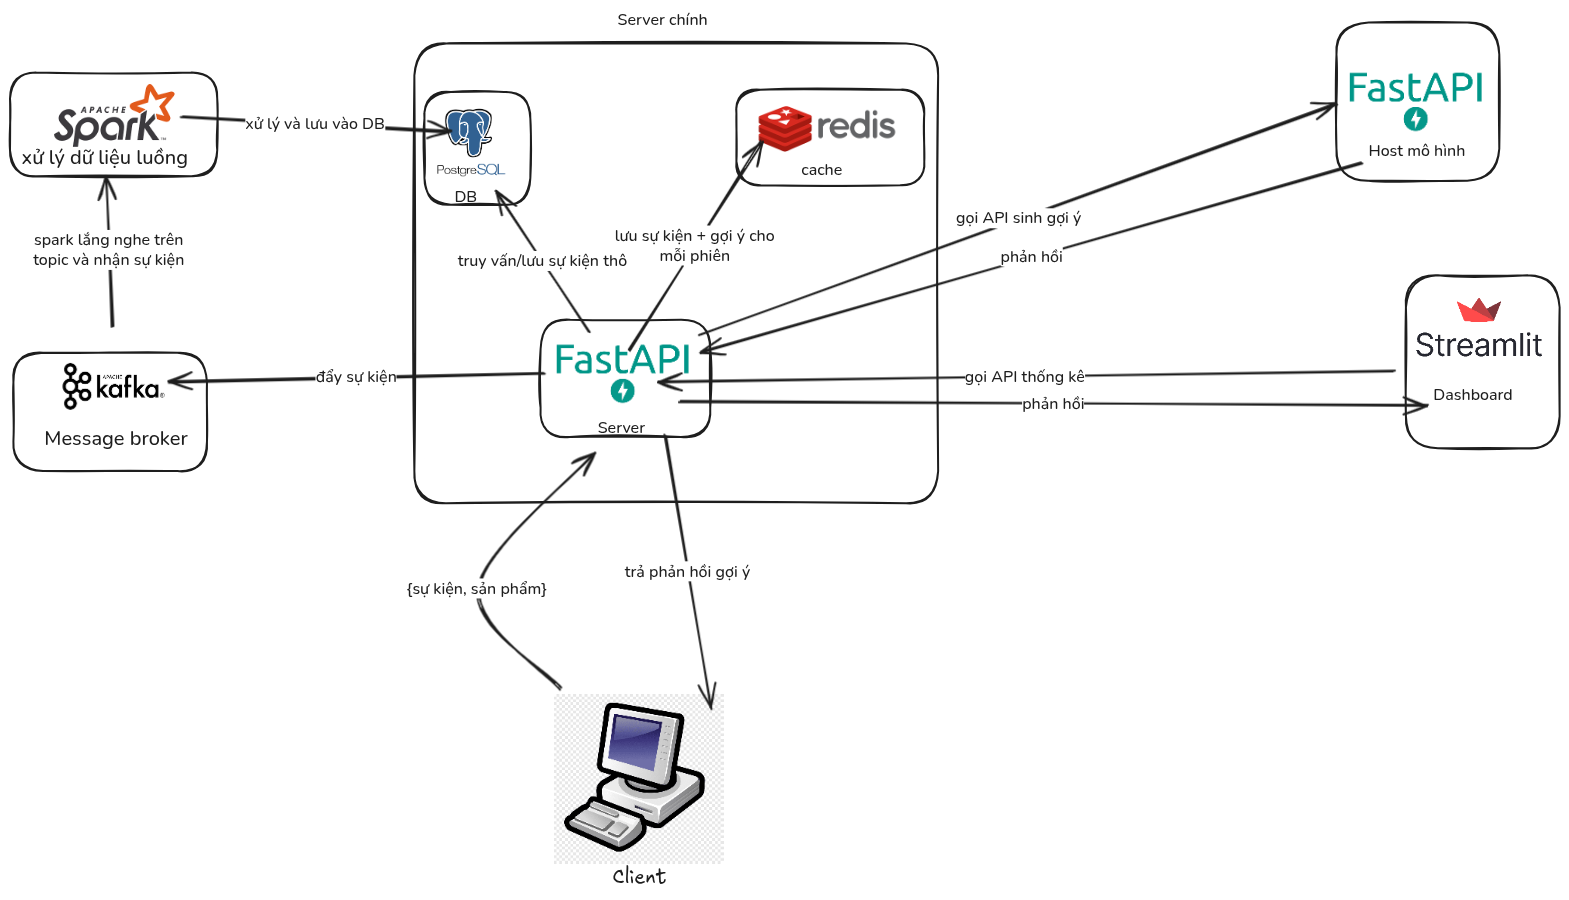
\includegraphics[width=0.9\textwidth]{../Hinhve/system-kpdll.png}
\caption{Kiến trúc tổng quan hệ thống xử lý dữ liệu}
\label{fig:architecture}
\end{figure}

\subsection{Hệ thống xử lý dữ liệu}

\subsubsection{Tiếp nhận và xử lý sự kiện}
API service được xây dựng bằng FastAPI, tiếp nhận các tương tác người dùng thông qua điểm cuối (endpoint) \textbf{POST /api/event}. Mỗi sự kiện bao gồm bốn trường:
\begin{itemize}
    \item \textbf{session\_id} - định danh phiên
    \item \textbf{aid} - mã sản phẩm
    \item \textbf{type} - loại tương tác (clicks, carts, orders)
    \item \textbf{ts} - thời gian Unix timestamp (mili-giây)
\end{itemize}
Khi nhận được sự kiện, API service thực hiện các bước sau:

\begin{enumerate}
    \item \textbf{Lưu vào Redis:} Sự kiện được thêm vào cuối danh sách (list) của phiên tương ứng trong Redis. Khóa có dạng phiên và được thiết lập thời gian sống (TTL) là 30 phút. Redis List là cấu trúc dữ liệu phù hợp cho việc lưu chuỗi sự kiện theo thứ tự thời gian, hỗ trợ thao tác thêm ở cuối và đọc toàn bộ với độ phức tạp O(1). Thao tác này trả về độ dài hiện tại của phiên - tham số quan trọng cho bước định tuyến mô hình.
    \item \textbf{Tra cứu gợi ý từ Redis (Read-Path):} Đây là bước then chốt trong kiến trúc Read-Path. API service kiểm tra bộ nhớ đệm Redis trước:
\begin{itemize}
    \item \textbf{Cache HIT:} Nếu đã có kết quả gợi ý được tính toán trước đó, trả về ngay lập tức cho người dùng. Model được sử dụng là ``cached''. Đây là trường hợp phổ biến nhất, đảm bảo độ trễ phản hồi ở mức miligây.
    \item \textbf{Cache MISS:} Nếu chưa có, API service truy vấn ma trận covisitation từ Redis để lấy danh sách sản phẩm liên quan cho từng sản phẩm trong phiên, sau đó tổng hợp và xếp hạng theo điểm số. Toàn bộ quy trình chỉ cần một round-trip đến Redis thông qua pipeline, đảm bảo độ trễ thấp.
\end{itemize}
Luồng Read-Path được thiết kế để luôn trả về kết quả cho người dùng ngay lập tức, không chờ đợi bất kỳ mô hình nào. Điều này giúp duy trì thời gian phản hồi ổn định bất kể trạng thái của hệ thống gợi ý.
    \item \textbf{Đẩy task tái tính toán nền (Write-Path):} Nếu độ dài phiên lớn hơn hoặc bằng 5 sự kiện, API service đẩy thông tin phiên vào hàng đợi \textbf{background\_queue} để worker nền thực thi. Tác vụ này chạy bất đồng bộ, không chặn luồng phản hồi chính. Các phiên ngắn (dưới 5 sự kiện) không cần tái tính toán vì covisitation đã đủ tốt.
    \item \textbf{Xuất bản lên Kafka:} Sự kiện được gửi bất đồng bộ lên topic của Kafka với thông tin bao gồm mã phiên, mã sản phẩm, loại tương tác, thời gian và mô hình được sử dụng. Việc gửi bất đồng bộ đảm bảo API không bị chặn bởi thao tác I/O của Kafka, giữ thời gian phản hồi ở mức thấp.
    \item \textbf{Đệm (buffer) vào PostgreSQL:} Sự kiện thô và thông tin dự đoán được đẩy vào các hàng đợi bộ đệm Redis. Một tác vụ nền chạy định kỳ sẽ đẩy toàn bộ bộ đệm vào PostgreSQL theo lô. Cơ chế này giảm tải kết nối database và tránh tạo quá nhiều transaction nhỏ lẻ.
    \item \textbf{Theo dõi độ chính xác:} Nếu sự kiện là carts hoặc orders, hệ thống kiểm tra xem sản phẩm người dùng tương tác có nằm trong danh sách gợi ý vừa trả về không, và ghi kết quả để tính toán tỷ lệ trúng (hit rate) và các metric đánh giá (Recall@K, NDCG@K, MRR@K).
\end{enumerate}

\subsubsection{Tái tính toán nền (Background Recompute)}
Worker nền chạy liên tục, nhận các task từ hàng đợi và thực thi theo chiến lược sau:

\begin{enumerate}
    \item \textbf{Phiên ngắn (dưới 5 sự kiện):} Gợi ý dựa trên covisitation từ Redis - không gọi mô hình từ xa.
    \item \textbf{Phiên dài (từ 5 sự kiện):} Gọi mô hình SASRec từ xa thông qua bộ ngắt mạch (circuit breaker). Nếu mô hình trả về kết quả thành công, kết quả được lưu vào bộ nhớ đệm Redis để các request tiếp theo đọc trực tiếp từ cache.
    \item \textbf{Mô hình thất bại:} Nếu SASRec quá thời gian (timeout) hoặc lỗi, hệ thống tự động chuyển sang dự phòng (fallback) bằng covisitation từ Redis. Nếu bộ ngắt mạch mở do lỗi liên tiếp, hệ thống bỏ qua gọi mô hình trong một khoảng thời gian để tránh quá tải.
\end{enumerate}

Kiến trúc Read-Path / Write-Path tách biệt mang lại ba lợi ích chính:
\begin{itemize}
    \item \textbf{Độ trễ thấp:} Người dùng luôn nhận kết quả từ Redis (ms) - nhanh hơn.
    \item \textbf{Khả năng phục hồi:} Khi mô hình từ xa gặp sự cố, Read-Path vẫn hoạt động bình thường với covisitation.
    \item \textbf{Tính đồng thời:} Worker nền có thể xử lý nhiều phiên song song mà không ảnh hưởng đến tốc độ phản hồi của API.
\end{itemize}

API service cũng cung cấp điểm cuối (endpoint) \textbf{GET /api/stats} phục vụ bảng điều khiển (dashboard) Streamlit, trả về tổng hợp các chỉ số:
\begin{itemize}
    \item Số phiên hoạt động.
    \item Thống kê dự đoán: tổng số, độ trễ (latency) trung bình, phân bố model usage.
    \item Tỷ lệ chuyển đổi funnel.
    \item Tỷ lệ trúng (hit rate).
    \item Metric Spark và các log bất thường.
\end{itemize}

Ngoài ra, API service triển khai ba tác vụ nền chạy định kỳ:
\begin{itemize}
    \item \textbf{Tái tính toán gợi ý:} Tính toán lại gợi ý cho các phiên dài, lưu kết quả vào cache.
    \item \textbf{Đồng bộ dữ liệu:} Đọc dữ liệu từ các bộ đệm Redis và ghi hàng loạt vào PostgreSQL.
    \item \textbf{Làm mới thứ hạng:} Tính toán lại thứ hạng cho các sản phẩm phổ biến.
\end{itemize}
Việc dọn dẹp (cleanup) dữ liệu cũ được thực hiện bởi một container riêng (docker-compose service \textbf{cleanup}), chạy script SQL xóa dữ liệu cũ hơn 30 ngày, kích hoạt thủ công hoặc qua cron job bên ngoài.

\subsubsection{Truyền tải luồng sự kiện}
Kafka đóng vai trò trung gian giữa API service và Spark Streaming, đảm bảo tính bất đồng bộ và khả năng phục hồi của pipeline. Hệ thống sử dụng Apache Kafka chạy ở chế độ KRaft với một topic duy nhất cho luồng sự kiện người dùng.

Producer (API service) được cấu hình để tối ưu hiệu năng: chỉ cầnleader ghi nhận thành công (không cần tất cả replica xác nhận), gom tin nhắn thành batch trước khi gửi, và sử dụng \textbf{session\_id} làm khóa phân vùng để đảm bảo các sự kiện cùng phiên được ghi vào cùng một partition, duy trì thứ tự xử lý. Việc gửi tin nhắn được thực hiện bất đồng bộ qua background task của FastAPI, không chặn luồng phản hồi chính.

\subsubsection{Xử lý streaming với Spark Structured Streaming}
Spark Streaming đọc dữ liệu từ Kafka thông qua cơ chế đọc luồng (stream read) của Spark Structured Streaming. Mỗi lô nhỏ (micro-batch) được kích hoạt với khoảng kích hoạt (trigger interval) 10 giây và áp dụng cơ chế kiểm soát phản áp (backpressure) để giới hạn số bản ghi xử lý mỗi batch. Dữ liệu thô dạng JSON được phân tích cú pháp (parse) với lược đồ (schema) cố định gồm các trường:
\begin{itemize}
    \item \textbf{session\_id}
    \item \textbf{aid}
    \item \textbf{type}
    \item \textbf{ts}
    \item \textbf{model\_used}
\end{itemize}

Spark áp dụng mốc thời gian (watermark) 2 phút trên trường dấu thời gian (timestamp) - các sự kiện đến trễ hơn 2 phút so với thời gian hiện tại sẽ bị loại bỏ. Ngưỡng này dung hòa giữa độ trễ của dữ liệu thời gian thực (dao động mạng (network jitter)) và nhu cầu giữ trạng thái (state) của các pipeline có cửa sổ (window).

Từ luồng dữ liệu đã được phân tích (parse), Spark thực hiện sáu pipeline phân tích song song thông qua cơ chế đa luồng (thread pool) trong hàm xử lý foreach batch:

\begin{enumerate}
    \item[\textbf{A.}] \textbf{Thống kê theo khoảng thời gian:} Tính toán các chỉ số tổng hợp theo cửa sổ (window) 1 phút: tổng số sự kiện, số phiên duy nhất (sử dụng thuật toán đếm xấp xỉ với sai số $\approx$2\%), số sản phẩm duy nhất, số sự kiện theo từng loại (click, cart, order), và tỷ lệ chuyển đổi click qua cart, cart qua order. Dữ liệu được ghi theo chế độ thêm (append) (mỗi cửa sổ (window) là một dòng mới). Bảng này phục vụ dashboard theo dõi xu hướng theo thời gian và phát hiện bất thường về lưu lượng.

    \item[\textbf{B.}] \textbf{Phát hiện bất thường:} Phát hiện phiên có dấu hiệu bot dựa trên ngưỡng động. Với mỗi phiên, pipeline tính số sự kiện trung bình mỗi phút; nếu vượt quá ngưỡng (\textit{mean} + $3 \times \textit{std}$) thì ghi nhận là bất thường. Các phiên bất thường được ghi vào bảng giám sát để phục vụ lọc nhiễu về sau.

    \item[\textbf{C.}] \textbf{Độ phổ biến thời gian thực:} Tính toán số lần xuất hiện lũy kế (cumulative) của từng sản phẩm theo loại sự kiện, sử dụng phép gom nhóm toàn cục với chế độ cập nhật (update mode). Vì dữ liệu được tích lũy từ đầu phiên streaming, mỗi batch mới ghi đè giá trị đã tồn tại thay vì cộng dồn - tránh lỗi đếm trùng (double-counting). Hệ thống không áp dụng cửa sổ (window) cho pipeline này vì yêu cầu độ phổ biến "mọi thời điểm" (all-time). Do Spark Streaming không duy trì thứ tự sắp xếp khi cập nhật luồng, thứ hạng (rank) của từng sản phẩm được tính toán lại định kỳ bởi tác vụ nền làm mới (refresh) trong API service.

    \item[\textbf{D.}] \textbf{Hiệu suất sản phẩm:} Tính toán các chỉ số cho từng sản phẩm: tổng số click, cart, order, và tỷ lệ chuyển đổi click qua cart, click qua order, cart qua order. Pipeline áp dụng cửa sổ (window) 1 giờ để tránh trạng thái không giới hạn (unbounded state) trên mốc thời gian (watermark) - Spark sẽ loại bỏ các cửa sổ (window) cũ hơn mốc thời gian (watermark), kiểm soát bộ nhớ. Dữ liệu được ghi vào bảng hiệu suất sản phẩm bằng cơ chế ghi đè, với khóa chính là mã sản phẩm.

    \item[\textbf{E.}] \textbf{Thống kê funnel theo mô hình:} Theo dõi hiệu suất của từng mô hình gợi ý thông qua các chỉ số: số phiên sử dụng mô hình, số phiên có click/cart/order, tỷ lệ chuyển đổi click qua order. Thông tin mô hình được API service nhúng trực tiếp vào tải trọng (payload) Kafka và Spark phân tích (parse) từ JSON - khác với cách tiếp cận cũ là join với bảng log dự đoán gây ra hai vấn đề: tình trạng tranh chấp (race condition) (Streaming xử lý sự kiện trước khi API ghi log) và quét toàn bộ bảng (full table scan) mỗi lô nhỏ (micro-batch).

    \item[\textbf{F.}] \textbf{Phân loại phiên:} Phân loại mỗi phiên thành ba nhóm dựa trên hành vi:
\begin{itemize}
    \item \textbf{buyer}: phiên có ít nhất một order.
    \item \textbf{cart\_abandoner}: phiên có cart nhưng không có order.
    \item \textbf{browse\_only}: phiên chỉ có click.
\end{itemize} Với mỗi nhóm, pipeline tính toán số phiên, độ dài trung bình, thời gian trung bình và tỷ lệ phần trăm trên tổng số phiên. Tỷ lệ phần trăm được tính trong Python (thay vì SQL) để tránh tình trạng tranh chấp (race condition) khi ghi đè đồng thời nhiều dòng.
\end{enumerate}

Tất cả sáu pipeline ghi kết quả vào PostgreSQL với chế độ batch và điểm phục hồi (checkpoint) để đảm bảo khả năng phục hồi cùng ngữ nghĩa chính xác-một-lần (exactly-once).

\subsubsection{Xử lý batch}
Bên cạnh xử lý streaming, hệ thống có các tác vụ batch chạy một lần thông qua container \textbf{setup-jobs} khi khởi tạo:

\begin{itemize}
    \item \textbf{Tạo topic Kafka:} Tạo topic trên Kafka với cấu hình partition và replication factor phù hợp.
    \item \textbf{Phân tích funnel:} Đọc dữ liệu lịch sử từ file dữ liệu OTTO trên Kaggle, tính toán tỷ lệ chuyển đổi funnel toàn cục, phân loại phiên và thống kê funnel theo mô hình. Dữ liệu được ghi vào các bảng phân tích với chế độ ghi đè (overwrite).
    \item \textbf{Khởi tạo sản phẩm phổ biến:} Tính toán top 100 sản phẩm phổ biến nhất theo từng loại sự kiện (clicks, carts, orders) từ dữ liệu lịch sử, ghi vào bảng sản phẩm phổ biến. Dữ liệu này được sử dụng cho chiến lược gợi ý nguội (cold start) khi phiên có ít hơn 3 sự kiện
\end{itemize}

Các batch job sử dụng chế độ ghi đè (overwrite) để đảm bảo dữ liệu sạch mỗi lần chạy. Dữ liệu đầu ra được lưu trực tiếp vào PostgreSQL.

\subsubsection{Lưu trữ dữ liệu}
Hệ thống sử dụng PostgreSQL làm kho dữ liệu phân tích chính với 12 bảng được tổ chức theo các nhóm chức năng:

\begin{itemize}
    \item \textbf{Dữ liệu sự kiện thô:} Lưu toàn bộ sự kiện để phục vụ retrain và rebuild matrices sau này.
    \item \textbf{Dữ liệu dự đoán:} Ghi lại mỗi lần dự đoán gồm model sử dụng, độ dài phiên, danh sách sản phẩm đề xuất, và thời gian xử lý (latency).此外 còn lưu kết quả kiểm tra độ chính xác (sản phẩm người dùng tương tác có nằm trong danh sách gợi ý không) và các metric đánh giá như Recall@K, NDCG@K, MRR@K theo từng sự kiện phiên.
    \item \textbf{Dữ liệu phân tích streaming:} Thống kê theo cửa sổ thời gian, hiệu suất từng sản phẩm, phân loại phiên, độ phổ biến theo thời gian thực, funnel theo mô hình.
    \item \textbf{Dữ liệu phân tích batch:} Tỷ lệ chuyển đổi toàn cục từ batch job.
    \item \textbf{Giám sát:} Phát hiện phiên bất thường, hiệu suất Spark (tốc độ xử lý, thời gian batch).
\end{itemize}

Cơ sở dữ liệu áp dụng chính sách lưu trữ (retention period): dữ liệu phân tích và log sự kiện thô được giữ 30 ngày, xóa bởi container cleanup chạy định kỳ.

Redis được sử dụng cho bốn mục đích chính:
\begin{itemize}
    \item \textbf{Lưu phiên:} Danh sách sự kiện theo thứ tự thời gian cho mỗi phiên.
    \item \textbf{Bộ nhớ đệm kết quả gợi ý:} Kết quả gợi ý của mỗi phiên được lưu để Read-Path trả về nhanh.
    \item \textbf{Ma trận covisitation:} Ma trận liên kết sản phẩm được preload từ file Parquet vào Redis.
    \item \textbf{Hàng đợi bộ đệm:} Đệm dữ liệu trước khi ghi vào PostgreSQL.
\end{itemize}

\section{Triển khai}
Toàn bộ hệ thống được đóng gói bằng Docker và Docker Compose, mỗi thành phần chạy trên một container riêng biệt và giao tiếp qua mạng nội bộ.

Spark có thể chạy ở hai chế độ: cục bộ (local), Spark chạy trực tiếp trên container xử lý streaming mà không cần cụm; hoặc cụm (cluster), tác vụ được gửi lên spark-master và phân bổ cho các worker node để xử lý song song. Mỗi worker được cấp tài nguyên CPU và RAM thông qua cơ chế giới hạn tài nguyên của container.


\section{Kết quả thực nghiệm}

\subsection{Hệ thống xử lý dữ liệu lớn}
Hệ thống được đánh giá thông qua bốn phép đo: thông lượng Kafka (Kafka throughput), kiểm tra tải API (API load test), độ ổn định Spark Streaming (Spark Streaming stability), và độ trễ đầu cuối (end-to-end latency).

SLA (Service Level Agreement) là các cam kết về mức độ dịch vụ mà hệ thống cần đạt được, hay đơn giản hơn là mục tiêu các chỉ số của hệ thống. Mỗi chỉ số KPI được đánh giá theo ba mức:
\begin{itemize}
    \item \textbf{OK} - đáp ứng yêu cầu, hệ thống hoạt động ổn định.
    \item \textbf{WARN} - cần theo dõi, có nguy cơ suy giảm hiệu năng.
    \item \textbf{FAIL} - không đạt, cần can thiệp ngay.
\end{itemize}
Các ngưỡng SLA cụ thể cho từng KPI:
\begin{itemize}
    \item Thông lượng Kafka (Kafka producer TPS):
    \begin{itemize}
        \item OK: $>$200K bản ghi/giây
        \item WARN: $>$100K bản ghi/giây
        \item FAIL: $<$50K bản ghi/giây
    \end{itemize}
    \item Độ trễ P95 của API (API P95 latency):
    \begin{itemize}
        \item OK: $<$200 ms
        \item WARN: $<$500 ms
        \item FAIL: $>$1 giây
    \end{itemize}
    \item Tỷ lệ lỗi API (API error rate):
    \begin{itemize}
        \item OK: $<$0,1\%
        \item WARN: $<$1\%
        \item FAIL: $\ge$5\%
    \end{itemize}
    \item Độ trễ P95 của Kafka (Kafka P95 latency):
    \begin{itemize}
        \item OK: $<$500 ms
        \item WARN: $<$5 giây
        \item FAIL: $\ge$5 giây
    \end{itemize}
    \item Độ ổn định Spark (Spark stability ratio):
    \begin{itemize}
        \item OK: $<$0,5
        \item WARN: $<$0,8
        \item FAIL: $\ge$1,0
    \end{itemize}
    \item Thời gian batch Spark (Spark batch duration):
    \begin{itemize}
        \item OK: $<$5 giây
        \item WARN: $<$8 giây
        \item FAIL: $>$10 giây
    \end{itemize}
    \item Độ trễ P50 đầu cuối (E2E P50 latency):
    \begin{itemize}
        \item OK: $<$10 giây
        \item WARN: $<$30 giây
        \item FAIL: $>$60 giây
    \end{itemize}
    \item Độ trễ P95 đầu cuối (E2E P95 latency):
    \begin{itemize}
        \item OK: $<$30 giây
        \item WARN: $<$60 giây
        \item FAIL: $>$5 phút
    \end{itemize}
\end{itemize}

\subsubsection{Thông lượng Kafka (Kafka throughput)}
Đánh giá Kafka sử dụng công cụ \textbf{kafka-producer-perf-test.sh} với 200000 bản ghi, kích thước 1KB mỗi bản ghi:
\begin{itemize}
    \item Thông lượng (throughput): 12353 bản ghi/giây (12,06 MB/giây).
    \item Độ trễ trung bình: 2287 ms.
    \item Độ trễ P95: 3473 ms.
    \item Độ trễ tối đa: 3578 ms.
\end{itemize}
So với SLA: thông lượng 12353 bản ghi/giây rất xa ngưỡng OK ($>$200K), đạt FAIL. Nguyên nhân là tài nguyên CPU giới hạn trong container và tranh chấp I/O (I/O contention) giữa Kafka log và điểm phục hồi (checkpoint) Spark trên cùng ổ đĩa. Độ trễ P95 3473 ms ở mức WARN (dưới ngưỡng FAIL 5 giây), cải thiện 18\% so với lần đo trước (4254 ms) nhờ tối ưu cấu hình Spark giảm tải CPU.

\subsubsection{Kiểm tra tải API (API load test)}
Kiểm tra tải API sử dụng k6 với kịch bản tăng tải ba giai đoạn (10, 50, 100 người dùng đồng thời, mỗi giai đoạn 3 phút), thời gian suy nghĩ (think time) 300-1300 ms giữa các yêu cầu:
\begin{itemize}
    \item Độ trễ trung vị (P50): 102 ms.
    \item Độ trễ trung bình: 1401 ms.
    \item Độ trễ P95: 5322 ms.
    \item Thông lượng: 22,2 yêu cầu/giây.
    \item Tỷ lệ lỗi (error rate): 0,76\%.
\end{itemize}
So với SLA: độ trễ P95 5322 ms vượt ngưỡng FAIL ($>$1 giây). Nguyên nhân chính là gọi API đến máy chủ (server) host mô hình quá thời gian (timeout) 2 giây - khi máy chủ mô hình hết thời gian chờ, API phải chuyển sang dự phòng (fallback), kéo độ trễ đuôi (tail latency) lên hàng giây. Trung vị chỉ 102 ms cho thấy hầu hết yêu cầu nhanh, nhưng độ trễ đuôi (tail latency) (P90-P95) bị ảnh hưởng nặng bởi bộ ngắt mạch (circuit breaker) mở. Tỷ lệ lỗi 0,76\% ở mức WARN (dưới ngưỡng FAIL 5\%), tăng so với 0,0\% ở lần đo trước do một số yêu cầu bị quá thời gian (timeout) khi fallback cũng thất bại.

\subsubsection{Độ ổn định Spark Streaming (Spark Streaming stability)}
Độ ổn định của Spark Streaming được đo bằng tỷ lệ ổn định (stability = thời gian xử lý / khoảng batch). Với khoảng kích hoạt (trigger interval) 10 giây:
\begin{itemize}
    \item Số batch xử lý: 23 batch.
    \item Thời gian batch trung bình: 14,8 giây.
    \item Thời gian batch tối đa: 35,4 giây (batch đầu do bắt kịp (catch-up)).
    \item Tốc độ xử lý trung bình: 690 dòng/giây, đạt đỉnh 1112 dòng/giây khi ổn định.
\end{itemize}
Tỷ lệ ổn định trung bình $\approx$1,48 (14,8s / 10s), ở mức FAIL ($>$1,0). Batch bắt kịp (catch-up) đầu tiên mất 35,4 giây để xử lý dữ liệu tồn từ Kafka. Sau khi ổn định, thời gian batch dao động 9-13 giây. Tốc độ xử lý tăng dần từ 282 dòng/giây (batch đầu) lên 1112 dòng/giây (batch 20), cho thấy hiệu quả của việc tối ưu cấu hình Spark. Spark chạy ở chế độ local (trên chính container spark-streaming), các worker node không tham gia xử lý.

\subsubsection{Độ trễ đầu cuối (End-to-end latency)}
Độ trễ đầu cuối đo thời gian từ lúc API nhận sự kiện đến khi dữ liệu xuất hiện trong PostgreSQL:
\begin{itemize}
    \item Độ trễ P50: 255 giây.
    \item Độ trễ P95: 428 giây (7 phút).
\end{itemize}
So với SLA: P50 255 giây và P95 428 giây đều vượt ngưỡng FAIL ($>$60 giây và $>$5 phút). Nguyên nhân là Spark xử lý chậm hơn tốc độ đầu vào do giới hạn số bản ghi mỗi batch, dù tốc độ xử lý đã cải thiện so với lần đo trước.

\subsubsection{Nhận xét}
Kết quả benchmark cho thấy hệ thống có những điểm đạt yêu cầu và những điểm cần cải thiện:

\begin{itemize}
    \item \textbf{Thông lượng Kafka (FAIL):} 12353 bản ghi/giây, rất xa ngưỡng $>$200K. Nguyên nhân chính là tài nguyên CPU giới hạn (4 lõi) trong môi trường container và tranh chấp I/O (I/O contention) giữa Kafka log và điểm phục hồi (checkpoint) Spark trên cùng ổ đĩa.

    \item \textbf{Độ trễ P95 Kafka (WARN):} 3473 ms, cải thiện 18\% so với lần đo trước (4254 ms) nhờ tối ưu cấu hình Spark giảm tải CPU. Dù vậy, vẫn cao hơn nhiều so với mức OK dưới 500 ms.

    \item \textbf{Độ trễ P95 API (FAIL):} 5322 ms, vượt ngưỡng $>$1 giây. Nguyên nhân chính là quá thời gian (timeout) khi gọi API máy chủ (server) mô hình (2 giây) - mỗi lần quá thời gian buộc API phải chuyển sang dự phòng (fallback), kéo độ trễ đuôi (tail latency) lên hàng giây. Trung vị chỉ 102 ms chứng tỏ hầu hết yêu cầu được xử lý nhanh, nhưng phân phối độ trễ có đuôi rất dài (tail latency): gap giữa P50 (102 ms) và P95 (5322 ms) lên tới 52 lần.

    \item \textbf{Tỷ lệ lỗi API (WARN):} 0,76\%, tăng từ 0,0\% ở lần đo trước. Một số yêu cầu bị quá thời gian (timeout) ngay cả khi fallback do tải cao. Dù vẫn dưới ngưỡng FAIL 5\%, đây là tín hiệu cần theo dõi.

    \item \textbf{Độ ổn định Spark (FAIL):} Tỷ lệ ổn định $\approx$1,48 (thời gian batch 14,8 giây trên khoảng kích hoạt (trigger interval) 10 giây), vượt ngưỡng FAIL ($>$1,0). Batch đầu mất 35,4 giây do bắt kịp (catch-up) lượng dữ liệu tồn từ Kafka. Sau đó, các batch dao động 9-13 giây, tốc độ xử lý tăng từ 282 lên 1112 dòng/giây nhờ cấu hình Spark được tối ưu. Spark chạy ở chế độ local (trên spark-streaming), các worker node không tham gia xử lý.

    \item \textbf{Thời gian batch Spark (FAIL):} Trung bình 14,8 giây, vượt ngưỡng $>$10 giây. Tuy nhiên, các batch sau ổn định ở 9-13 giây, cho thấy cải thiện so với lần đo trước nhờ điều chỉnh tài nguyên executor.

    \item \textbf{Độ trễ đầu cuối (FAIL):} P50 255 giây và P95 428 giây, tương đương lần đo trước. Nguyên nhân chính là Spark xử lý chậm hơn tốc độ đầu vào, dù tốc độ xử lý dòng/giây đã cải thiện nhờ cấu hình.
\end{itemize}

Tóm lại, các KPI đều ở mức FAIL hoặc WARN, chỉ ra ba nút thắt cổ chai (bottleneck) chính:
\begin{itemize}
    \item Tài nguyên CPU và tranh chấp I/O (I/O contention) hạn chế thông lượng Kafka và Spark.
    \item Quá thời gian (timeout) gọi máy chủ (server) mô hình kéo độ trễ API.
    \item Spark chưa chạy ở chế độ cụm (cluster mode) - các worker node không tham gia xử lý, toàn bộ tác vụ (task) chạy trên container xử lý streaming.
\end{itemize}

\end{document}
